%\kant[1-2]
\textbf{Density Functional Theory study of hydroxyl defects in LiFePO$_4$ and LiMnPO$_4$ cathode materials. }


\\
Cathode is the positive electrode in the batteries essential for their general electrochemical features.

Several materials have been used as a cathode part in the lithium-ion rechargeable batteries, but their electrochemical characteristics have not satisfied all user requests. 

LiFePO$_4$ and LiMnPO$_4$ materials have a high capacity, good operating voltage and cycle stability compared to other cathode polyanionic compounds.

\textit{DFT approach was used in the investigation of the hydroxyl defects structure within LiFePO$_4$ and LiMnPO$_4$ cathode material. The aim of current work is to establish the influence of OH defects on the structure of LiFePO$_4$ and LiMnPO$_4$ materials and their electronic properties. These properties need to be improved due to the poor electonic conductivity of LiFePO$_4$ and LiMnPO$_4$ materials in their pure form .}

The aim of current work is to establish the influence of OH defects on the structure of LiFePO$_4$ and LiMnPO$_4$ materials and their electronic properties. They need to be improved due to the poor electonic conductivity of LiFePO$_4$ and LiMnPO$_4$ materials in their pure form. \textit{DFT approach was used in the investigation. }

The structure of OH-defects in LiFePO$_4$ can not be determined from the experiment, therefore their computational study is required. The Density Functional Theory in the VASP code implementation is used to identify and study the defect structure of material on the atomic level. 

The current work established the equilibrium configuration of the hydroxyl group defect within LiFePO$_4$ and LiMnPO$_4$ materials. The molecular dynamic simulations were provided in order to achieve the full knowledge about the defect distribution at the certain temperatures. The thermodynamical analysis shows the appropriate of PO$_4$-O$_4$H$_4$ substitutional defect compared to the other positions. As a result, the impact of hydroxyl defect to the electronic properties of materials was established.

\textit{Investigation of the possible interstitial and substitutional hydrogen defects and potential energy surface of their possible positions in the combination with molecular dynamic simulations were provided in order to achieve the full knowledge about the defect distribution.} These defects have a huge influence on the batteries electrochemical characteristics and their study is critical for further material improvement. 


FIRST VERSION:
Material of LiFePO$_4$ is widely used as a cathode in rechargeable lithium-ion batteries and has several advantages compared to other polyanionic compounds. There is a high relative energy levels in Fe$^{3+}$/Fe$^{2+}$ redox couple - extreme valencies of Fe in LiFePO$_4$ and FePO$_4$, corresponding to full battery charge and discharge. Also LiFePO$_4$ is lower in toxicity and more inexpensive due to a wide distribution of iron. This material has a vast amount of interest in term of electrochemical application due to its relatively high capacity (till 170 mAhg$^{-1}$), good operating voltage (3.5V), leading to an energy density 578 Wh kg$^{-1}$ and cycle stability, \cite{franger2003comparison}. Although this material is well studied, investigation of defects in it is still very important and active topic. The defects have a huge influence on the electrochemical characteristics of the battery as a whole, and their study is critical for further material improvement.  

Along with well-known and investigated antisite Li-Fe defect and excess of Fe atom in Li-vacancy site the another type of defect - phosphorus deficiency can be observed in experiment \cite{amisse2015singular}. The former two of defects are unwelcome due to the blocking of the lithium diffusion pathways with subsequent reduction of the capacity \cite{hu2015molecular}, but they are fixed by post-preparation annealing process. The last one defect has relatively high energy of formation. The fact of its observation in an experiment in combination with hydroxyl groups as an impurity \cite{sumanov2019hydrotriphylites} suggests the compensation mechanism available, which is not well studied. The hydrothermal technique of sample preparation from the aqueous solutions with low concentration of LiFePO$_4$ precursors in water can be basis of the assumption of the substitutional hydrogen defect in place of phosphorus vacancy.  

The structure of OH-defects in LiFePO$_4$ cannot be determined from experiment, therefore their computational study is required. Accurate knowledge of hydrogen positions within the phosphorus vacancy as well as their formation energies can be obtained with density functional theory (DFT) computations. Thus, the aim of current work is to establish the influence of OH defects on the structure of LiFePO$_4$ material and its electronic properties. To achieve this goal the following task should be solved:\\
1. Comparison analysis of different vacancies and  interstitial hydrogen defects;\\
2. The energetic analysis of the positions of hydrogen atoms (by potential energy surface analysis for possible hydrogen distribution);\\
3. Molecular dynamics simulation of defective structure at the certain temperatures;\\
4. Thermodynamical comparison of substitutional defects at different atoms sites;\\
5. The influence of hydrogen substitutional defects on the electronic properties of material; \\
6. Comparison of results with references.



table chem pot:


\begin{table}[h]
\caption{Chemical potentials of species}
\label{tabular:LiFeP}
\begin{center}
\begin{tabular}{|c|c|}
\hline
&  \\
\textbf{Type of atom} & \textbf{$\mu (X)$ potential}, eV  \\
\hline
&  \\
H & -4.610 \\
\hline
&  \\
Li &  -5.821  \\
\hline
&  \\
Fe & -10.095 \\
\hline
&  \\
P &  -10.048 \\
\hline
\end{tabular}
\end{center}
\end{table}


\textbf{Interstitial} & \textbf{E$_{form}$, eV} & \textbf{Substitution} & \textbf{E$_{form}$, eV (GGA)} & \textbf{E$_{form}$, eV (GGA)} & \textbf{E$_{form}$, eV (GGA+U)} \\
\textbf{defect} & \textbf{(GGA)} & \textbf{defect} & \textbf{(GGA)} & \textbf{(GGA)} & \textbf{(GGA+U)} \\
 & $\mu(O_2)$=-11.52 eV &  & $\mu(O_2)$=-11.52 eV & $\mu(O_2)$=-13.1 eV & $\mu(O_2)$=-13.1 eV \\
 
Interstitial & E$_{form}$, eV & Substitution & E$_{form}$, eV (GGA) & E$_{form}$, eV (GGA) & E$_{form}$, eV (GGA+U) \\
defect & (GGA) & defect & (GGA) & (GGA) & (GGA+U) \\
 & $\mu(O_2)$=-11.52 eV &  & $\mu(O_2)$=-11.52 eV & $\mu(O_2)$=-13.1 eV & $\mu(O_2)$=-13.1 eV \\



\section{Electronic properties of defective structures}

The influence of phosphorus vacancy and substitution phosphorus by the hydrogen to electronic properties of material was investigated in the current work. The main disadvantage of LiFePO$_4$ and LiMnPO$_4$ is their poor electronic conductivity in the pure form. The carbon coating is used at the sample preparation stage to solve this problem and make material without band-gap in the Fermi level. Thus, the improvement of electronic properties of material is a crucial aim of its preparation. It can be affected by hydroxyl group defects due to the charge compensation mechanism. 

Firstly, the influence of phosphorus vacancy on the electronic conductivity can be considered in density of states study (Fig.\ref{ris:0DOS}).

\begin{figure}[ht]
\center{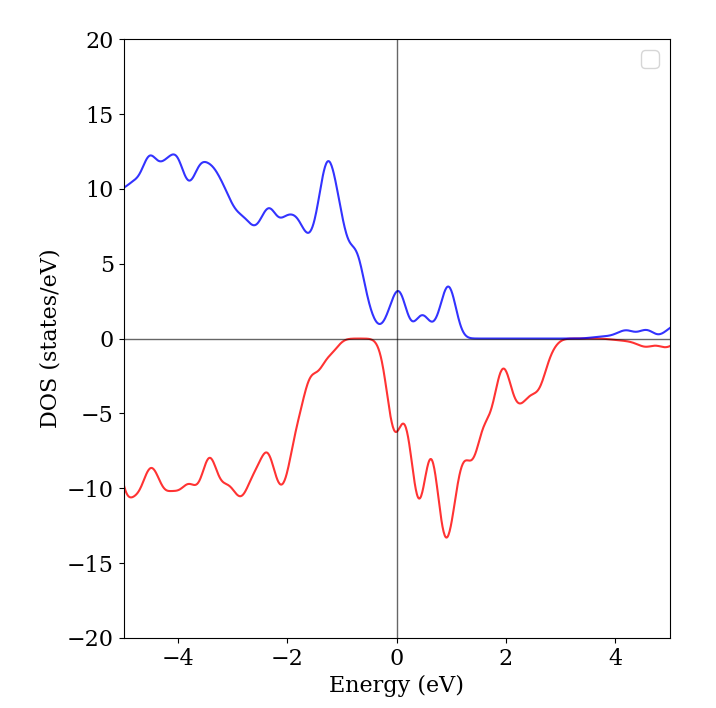
\includegraphics[width=0.6\linewidth]{pictures/0H_LFPdos.png})}
\caption{Density of electronic states for LiFePO$_4$ with P$_{vacancy}$}
\label{ris:0DOS}
\end{figure}

The influence of 1, 2, 3 or 4 hydrogen substitution atom in place of defective PO$_4$ place is presented in Fig.\ref{ris:1-4DOS}. The absence of band-gap at the Fermi level is clearly seen. All of these defective materials are conductors.

\begin{figure}[ht]
\begin{minipage}[h]{0.5\linewidth}
\center{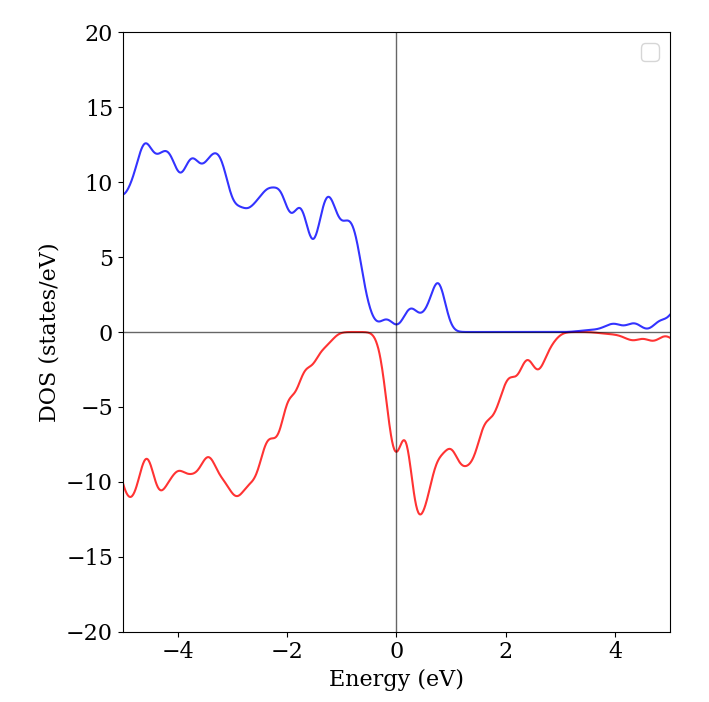
\includegraphics[width=1\linewidth]{pictures/1H_LFPdos.png} \\ a) PO$_4$-O$_4$H }
\end{minipage}
\hfill
\begin{minipage}[ht]{0.5\linewidth}
\center{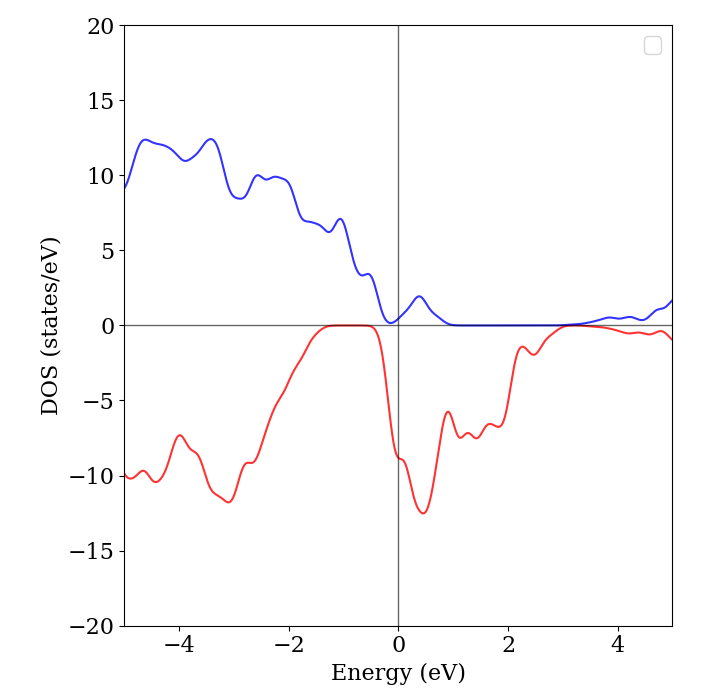
\includegraphics[width=1\linewidth]{pictures/2H_LFPdos.png} \\ b) PO$_4$-O$_4$H$_2$ }
\end{minipage}
\vfill
\begin{minipage}[h]{0.5\linewidth}
\center{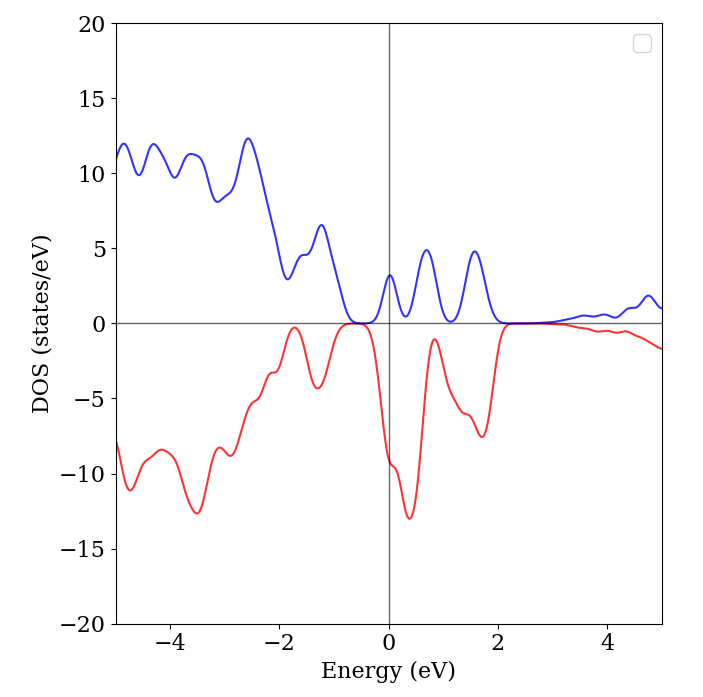
\includegraphics[width=1\linewidth]{pictures/3H_LFPdos.png} \\ c) PO$_4$-O$_4$H$_3$ }
\end{minipage}
\hfill
\begin{minipage}[ht]{0.5\linewidth}
\center{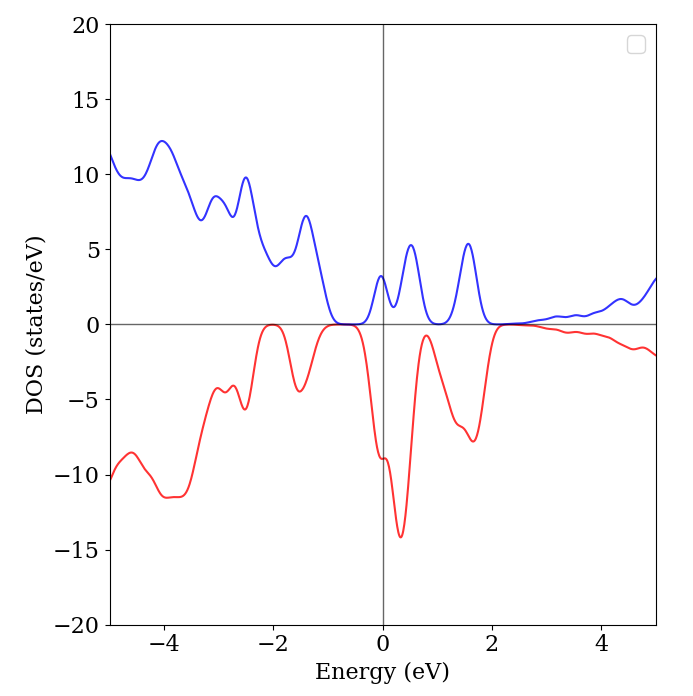
\includegraphics[width=1\linewidth]{pictures/4H_LFPdos.png} \\ d) PO$_4$-O$_4$H$_4$ }
\end{minipage}
\caption{DOS of LiFePO$_4$ with different defect composition }
\label{ris:1-4DOS}
\end{figure}

The same results of electronic density at the Fermi level can be obtained in case of hydroxyl group defects existing in LiMnPO$_4$ (Fig.\ref{ris:0DOS_LMP}). The influence of 1, 2, 3 or 4 hydrogen substitution atom in place of defective PO$_4$ place is presented in Fig.\ref{ris:1-4DOS_LMP}.

\begin{figure}[ht]
\center{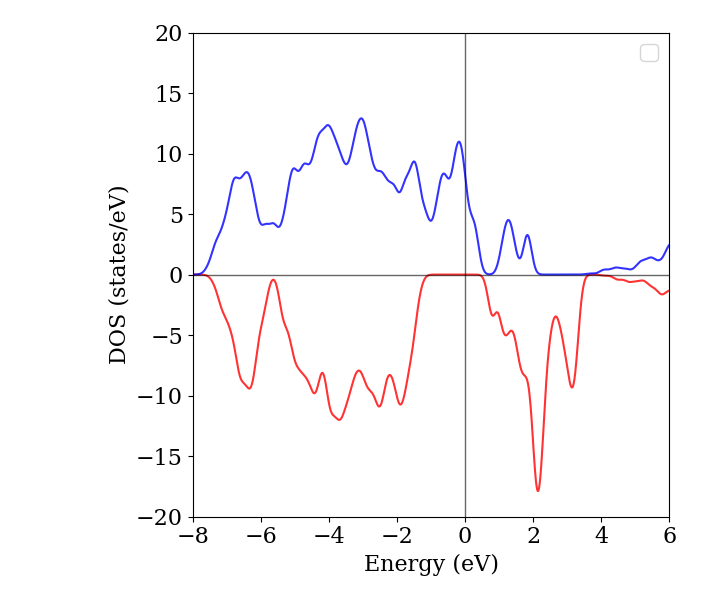
\includegraphics[width=0.6\linewidth]{pictures/0H.png} }
\caption{Density of electronic states for LiMnPO$_4$ with P$_{vacancy}$}
\label{ris:0DOS_LMP}
\end{figure}

\begin{figure}[ht]
\begin{minipage}[h]{0.5\linewidth}
\center{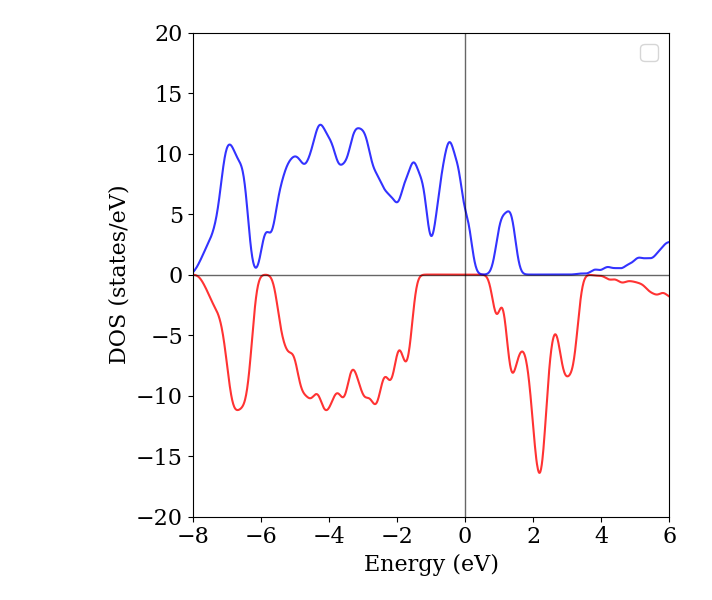
\includegraphics[width=1\linewidth]{pictures/1H.png} \\ a) PO$_4$-O$_4$H }
\end{minipage}
\hfill
\begin{minipage}[ht]{0.5\linewidth}
\center{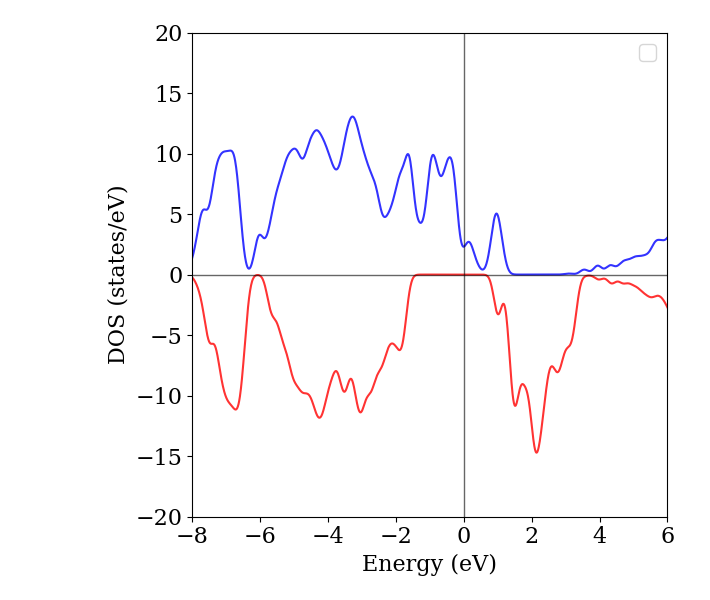
\includegraphics[width=1\linewidth]{pictures/2H.png} \\ b) PO$_4$-O$_4$H$_2$ }
\end{minipage}
\vfill
\begin{minipage}[h]{0.5\linewidth}
\center{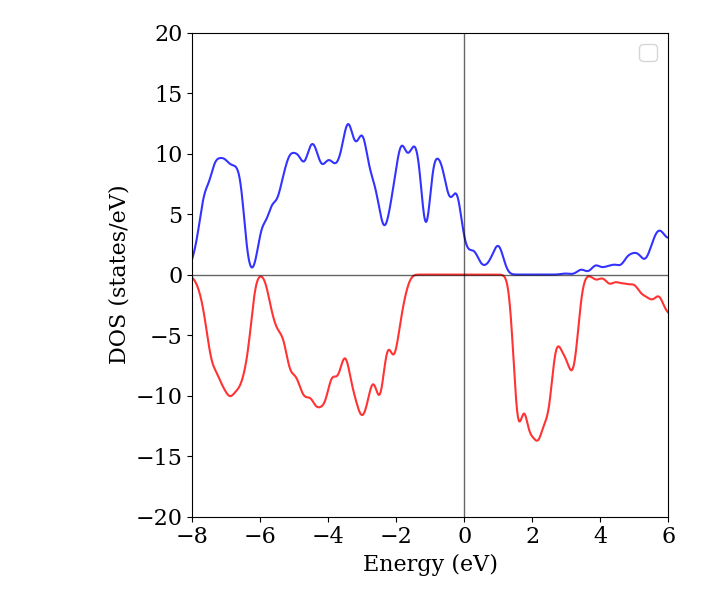
\includegraphics[width=1\linewidth]{pictures/3H.png} \\ c) PO$_4$-O$_4$H$_3$ }
\end{minipage}
\hfill
\begin{minipage}[ht]{0.5\linewidth}
\center{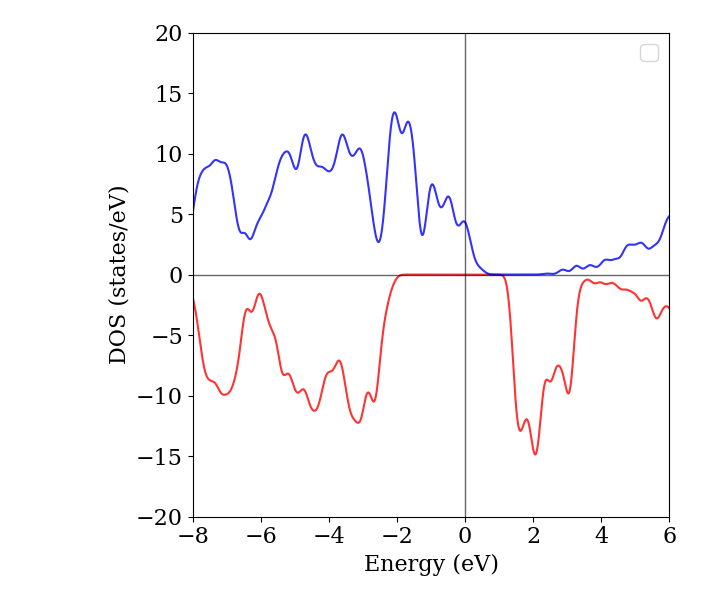
\includegraphics[width=1\linewidth]{pictures/4H_low.png} \\ d) PO$_4$-O$_4$H$_4$ }
\end{minipage}
\caption{DOS of LiMnPO$_4$ with different defect composition }
\label{ris:1-4DOS_LMP}
\end{figure}

\section{Comparison with references}

\begin{equation}
Li_{0.9}Fe_{0.03}^{3+}Fe_{1.07}^{2+}(PO_4)_{0.85}(OH)_{0.6}
\end{equation}

\begin{equation}
Li_{0.97}Fe_{0.05}^{3+}Fe_{0.99}^{2+}(PO_4)_{0.9}(OH)_{0.4}
\end{equation}

\begin{equation}
Li_{1.06}Fe_{0.95}PO_4
\end{equation}